\chapter{Graphical Indoor Positioning : the Android application}

 \section{Purpose of the android application}
The android application is the unique graphical interface the user can access for this project. It allows him to perform two operations: \\
\begin{itemize}
\item [$\rightarrow$] calibrate the program by sending a fingerprint of points to the server;
\item [$\rightarrow$] enjoy seeing his position travel across the map.
\end{itemize}
    ~\\
\indent Besides, we had in mind an application which allows to easily transmit calibration informations because creating a fingerprint map can quickly become fastidious for the user. \\
\indent Another aim was to make the graphical interface easy to handle for the user. This is done by creating a viewport which is an object that can be scaled, translated and rotated. The way it is handled looks like how google maps are handled (this way, the user already know how to perform the operations). \\
 
 \section{Architecture}
  Most of the work done in the architecture is naturally divided in two part :  
  \begin{itemize}
  \item[$\rightarrow$] Calibration side : everything related to the sending of a calibration position in order to make the fingerprint ;
  \item[$\rightarrow$] Location side : everything related to the reception of our current position.
  \end{itemize}
  ~\\
\indent Concerning the following class diagrams, their aim is to give an overall view of the architecture. The already implemented classes are not detailed and are represented in green. \\
  
  \begin{sidewaysfigure}
     \rotatebox{0}{
      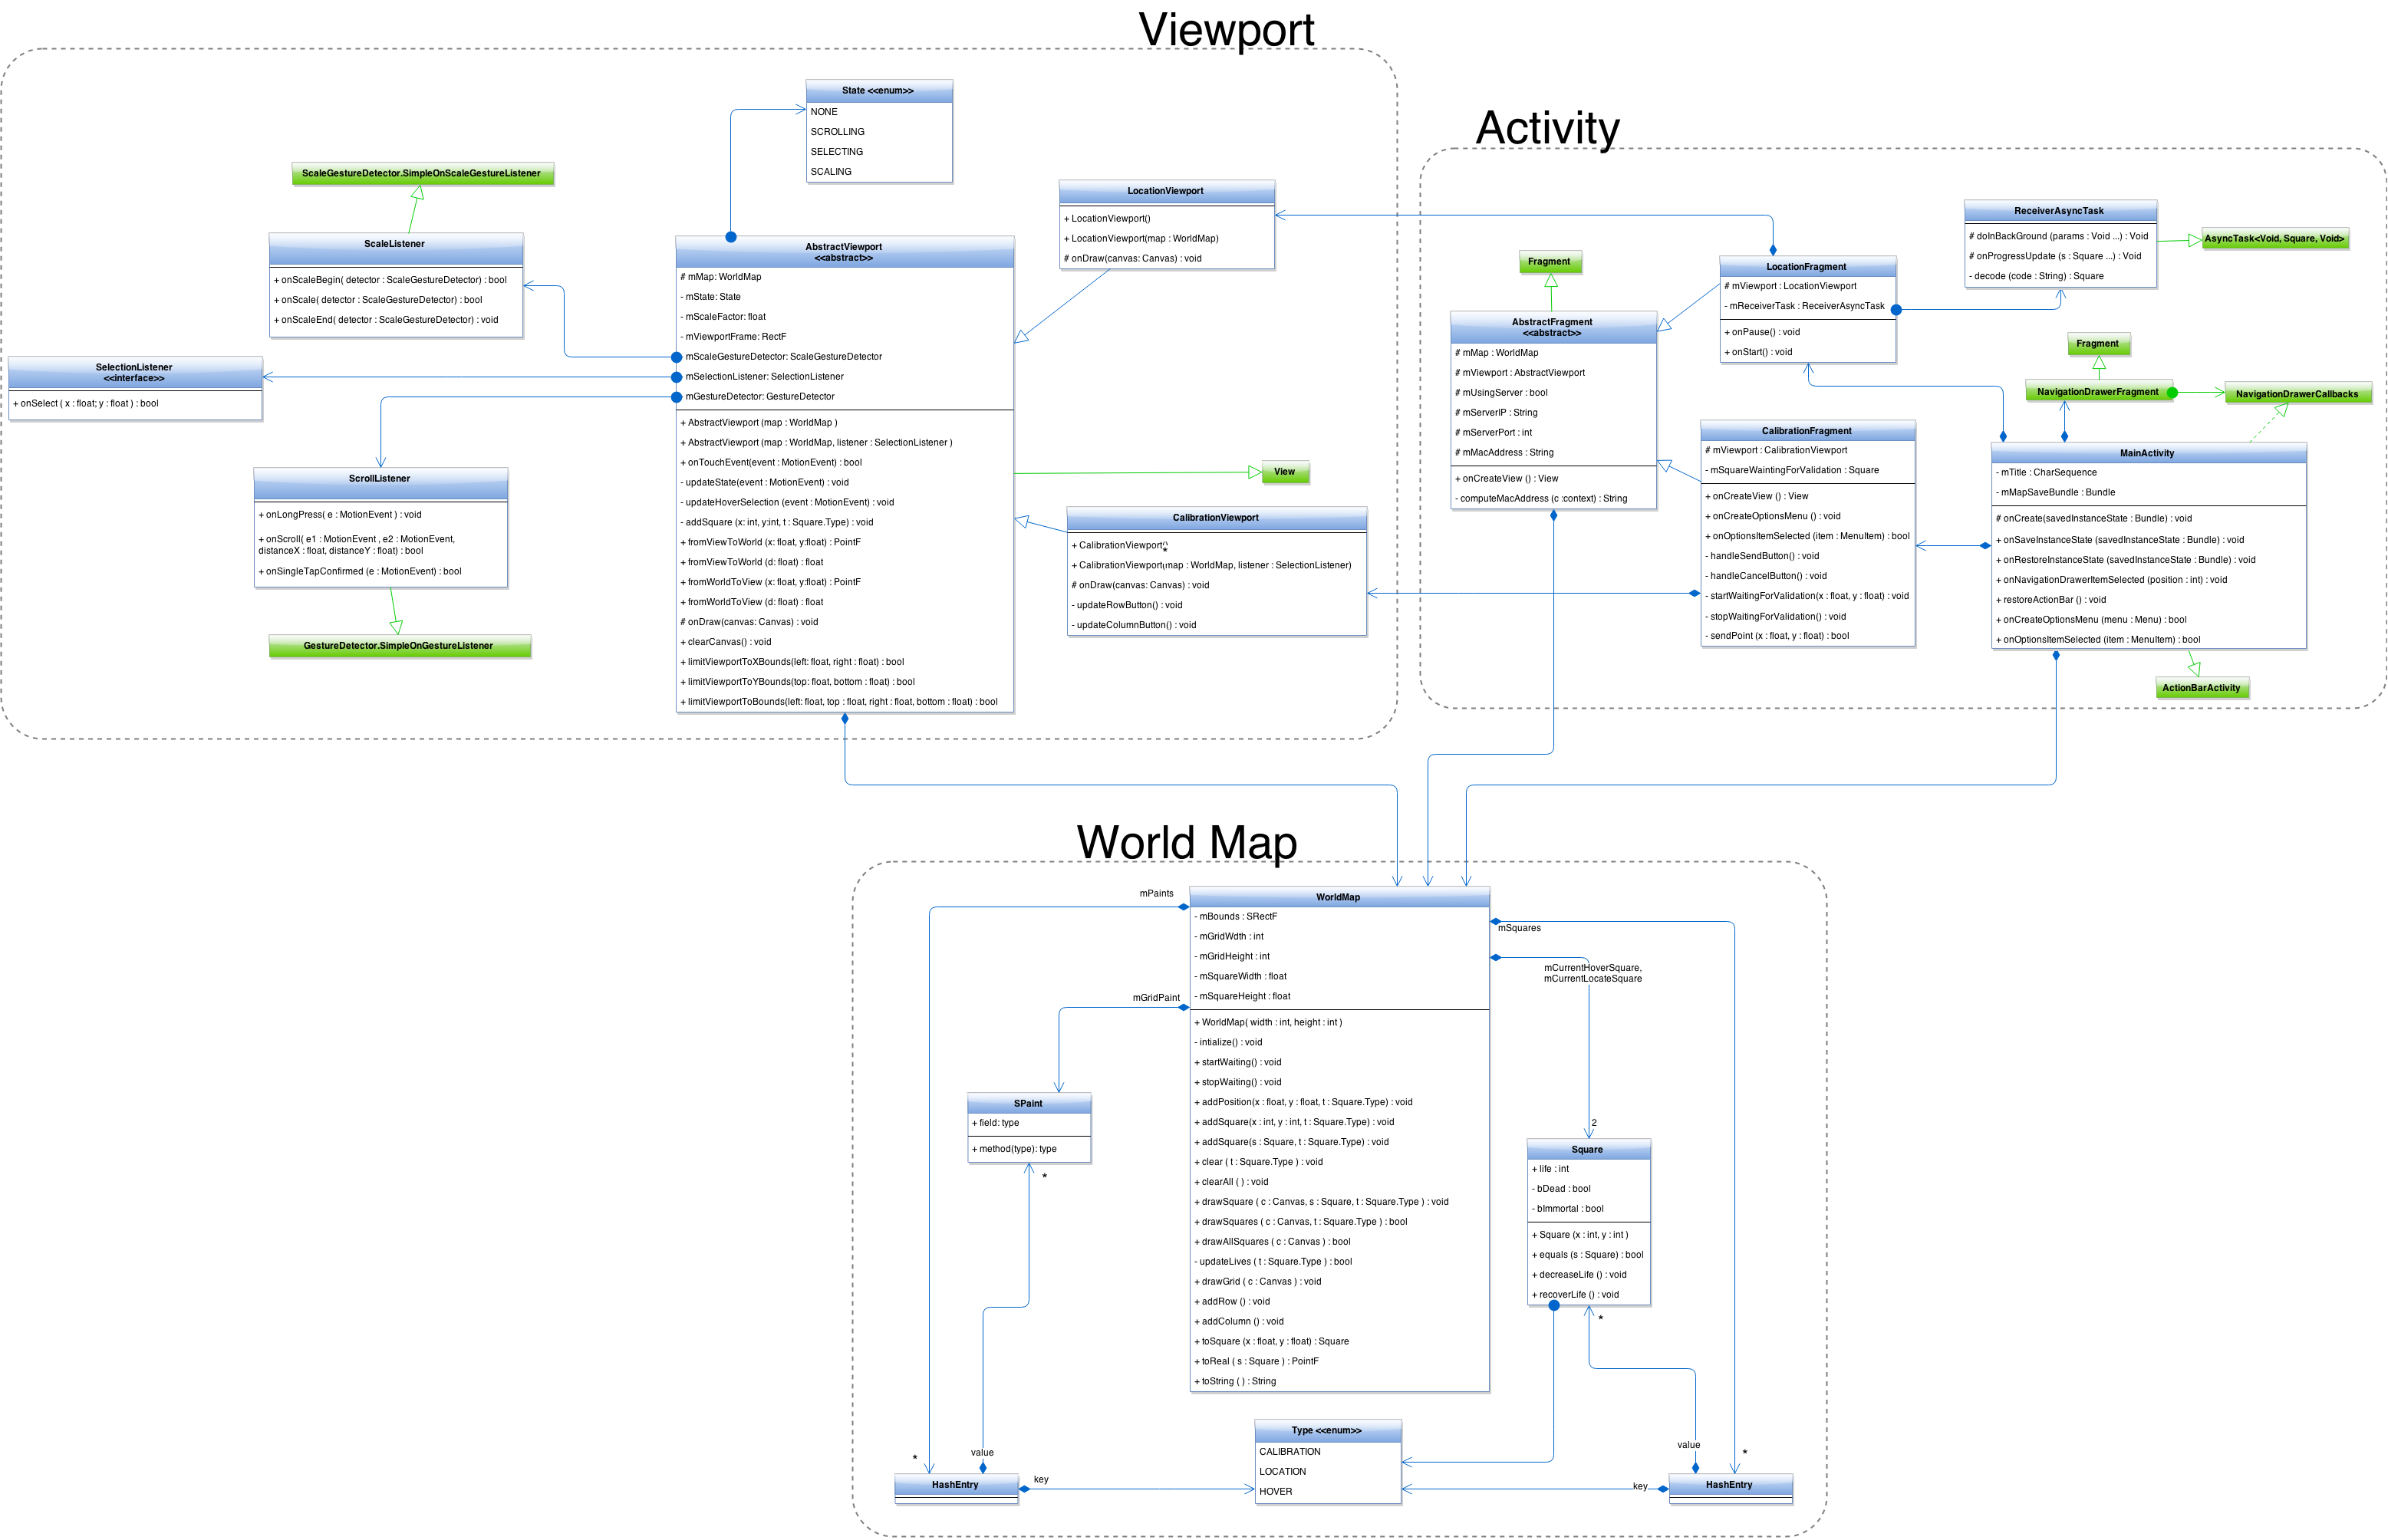
\includegraphics[scale = 0.23]{img/android/LO53_Android_Class} 
      }
     \caption{Android application global class diagram.}
     \label{fig:android_glob_class_diag}
    \end{sidewaysfigure}
  \newpage
    
   The global architecture can be divided into 3 main parts :
   \begin{itemize}
    \item[$\rightarrow$] The Activity part, which concerns everything related to the activity and the fragments (this is very common in android programming) ;
    \item[$\rightarrow$] The Viewport part which deals with the viewport (listening to translating or scaling events);
    \item[$\rightarrow$] The WorldMap part which consists in one class, the world map which is a shared object between the Activity and the Viewport part.
   \end{itemize}
   
  \subsection{Activity part}
   This part of the architecture is structured as something very specific to android : the Activity and its Fragments. \\

     \begin{figure}[H]
      \centering
       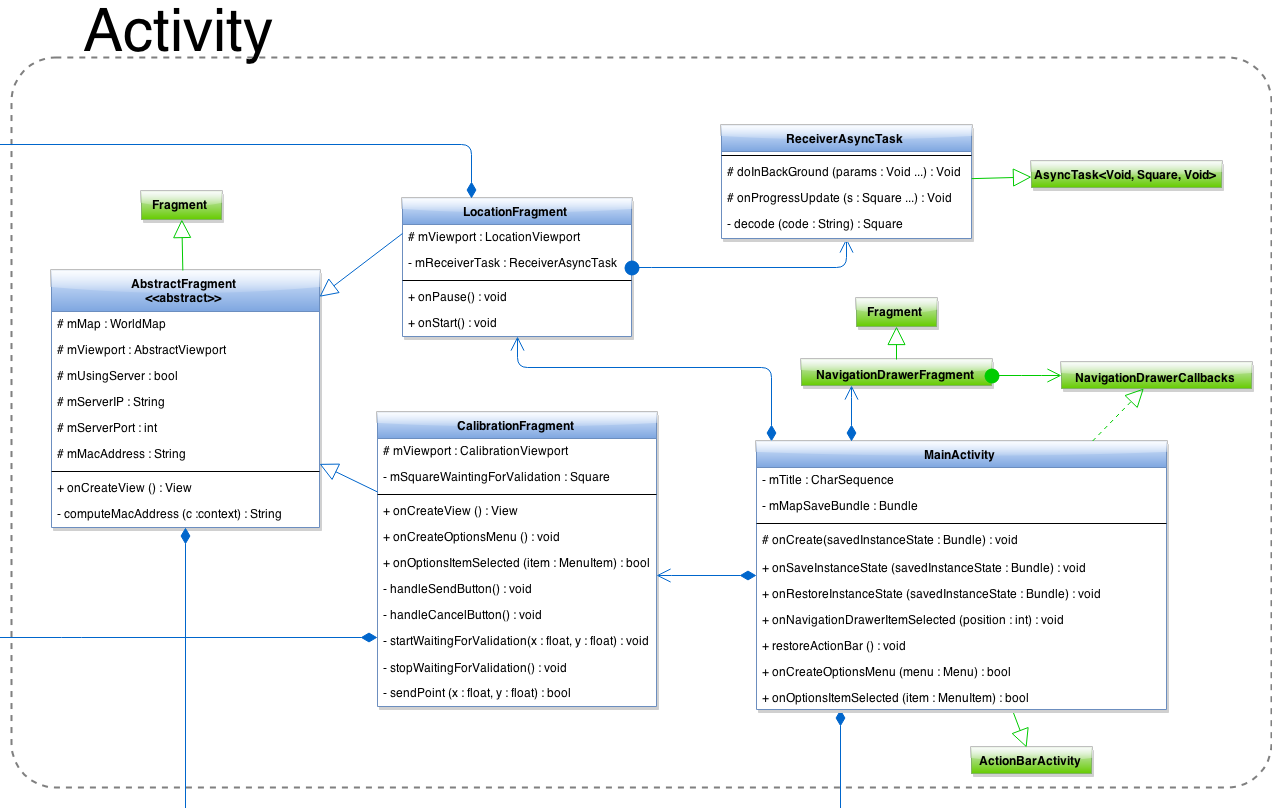
\includegraphics[scale = 0.35]{img/android/LO53_Android_Class_Activity}
      \caption{Activity class diagram.}
      \label{fig:android_activity_class_diag}
     \end{figure}
    ~\\
    
   The activity can be here assimilated as something near of a \textit{main()} function in classical programming. This is important to mention because it is not always the case with the android API. Most of the time, one activity is related to one operation the user can perform.\\
  It is made to handle four fragments : 
  \begin{itemize}
   \item[$\rightarrow$] the CalibrationFragment;
   \item[$\rightarrow$] the LocationFragment;
   \item[$\rightarrow$] the NavigationDrawerFragment : made for switching between the previous two ones ;
   \item[$\rightarrow$] the SettingsFragment.
  \end{itemize}
  ~\\
\indent The main activity is composed of an action bar and a container. The container can contain either the calibration, the location, or the settings fragment. 
%#TODO 
This is the navigation drawer fragment which handles the switch between possible contains of container.
%#ENDTODO   
The NavigationDrawerFragment is not detailed in the report because it is irrelevant considering the main purpose of the application, unlike both other fragments which represent the core. \\
\indent Moreover, the SettingsFragment was a last-minute inclusion so it does not appear in the class diagram. \\ 

\indent The LocationFragment and the CalibrationFragment extend both of an AbstractFragment which defines methods to be implemented such as :
   \begin{itemize}
   \item[$\rightarrow$] get the world map bundle;
   \item[$\rightarrow$] get the mobile phone mac address;
   \item[$\rightarrow$] fetch the server's ip  and the 'using server' boolean from the preferences.
   \end{itemize}
   ~\\
\indent How the location and calibration points are respectively received and sent using sockets is detailed in the third chapter of this report.
  \subsection{Viewport part}

  \begin{sidewaysfigure}
     \rotatebox{0}{
      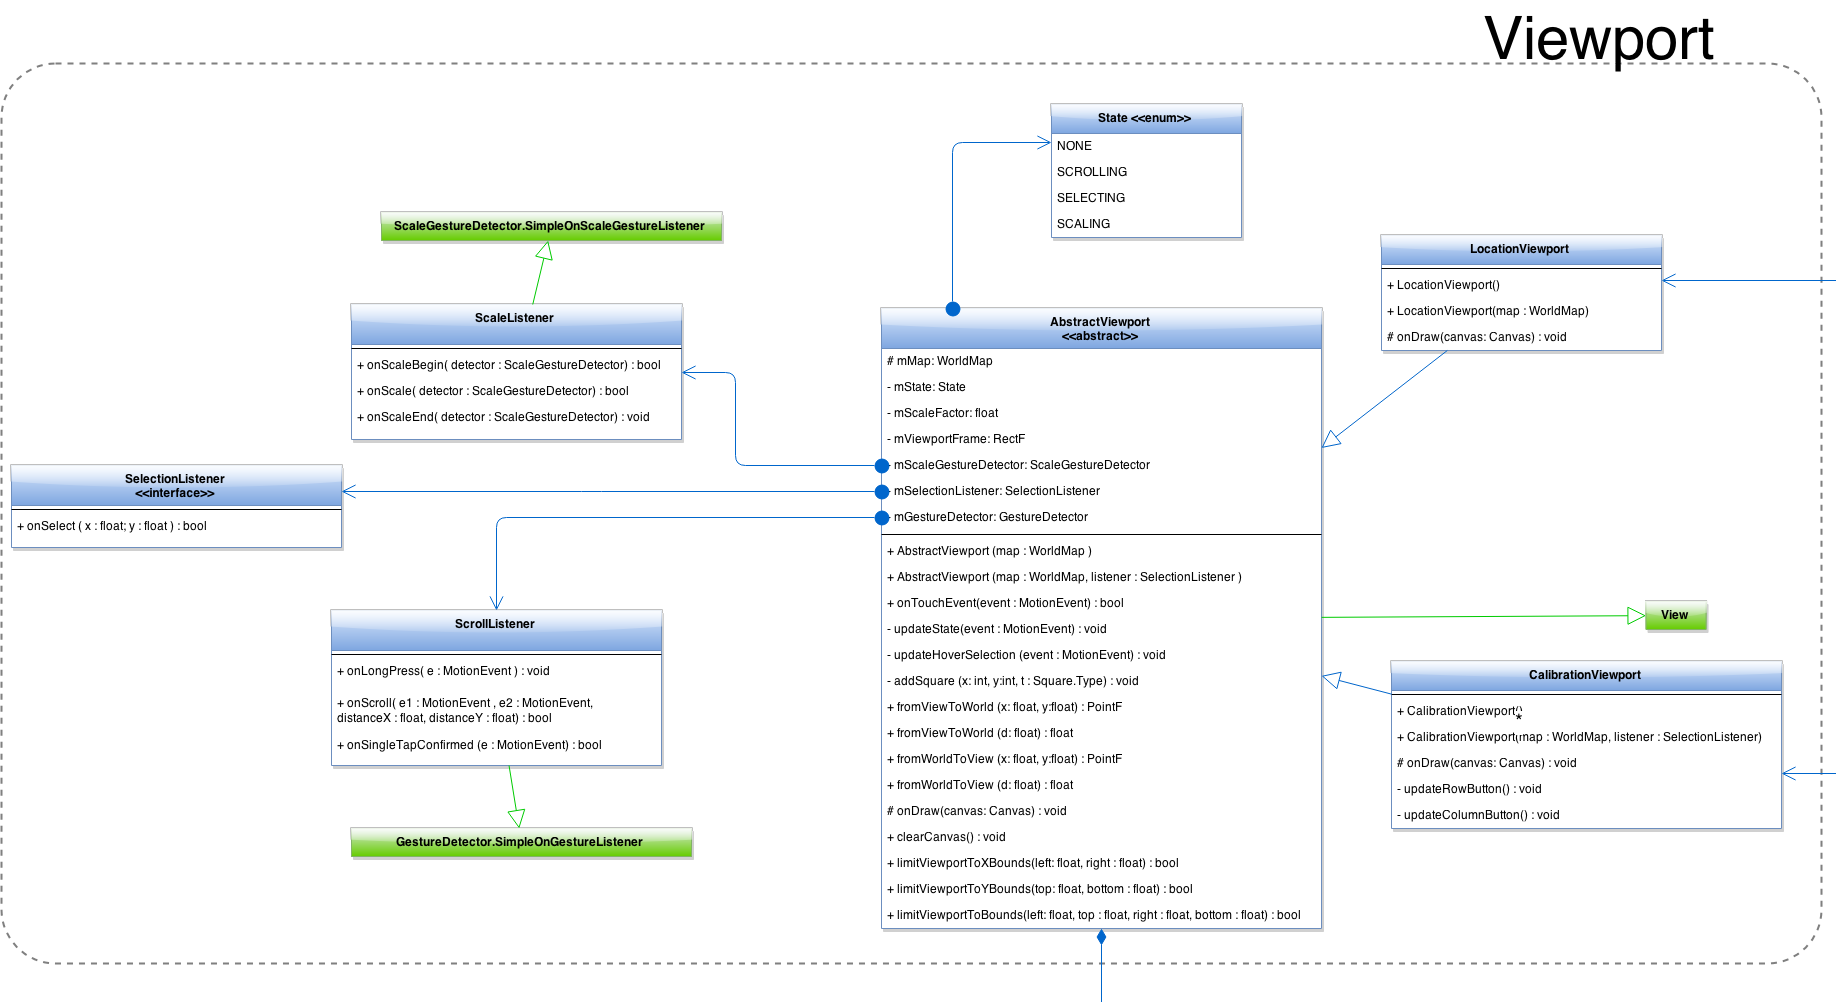
\includegraphics[scale = 0.38]{img/android/LO53_Android_Class_Viewport} }
     \caption{Activity class diagram.}
      \label{fig:android_viewport_class_diag}
     \end{sidewaysfigure}
    \newpage
   ~\\
    
\indent Just like for the fragments, an AbstractViewport class have been done. This is where the scaling and dragging behaviours are defined. The Location and Calibration fragments are just here to draw points and, in case of calibration, draw the "add row" and "add column" buttons.

\subsubsection {A state machine to handle finger's inputs}
    Creating a dynamic viewport is not an easy thing. The first we have to do is differentiate several states. All states are defined in an enumeration.
Here is a transition-state diagram which defines how inputs are handled.\\

     \begin{figure}[H]
      \centering
       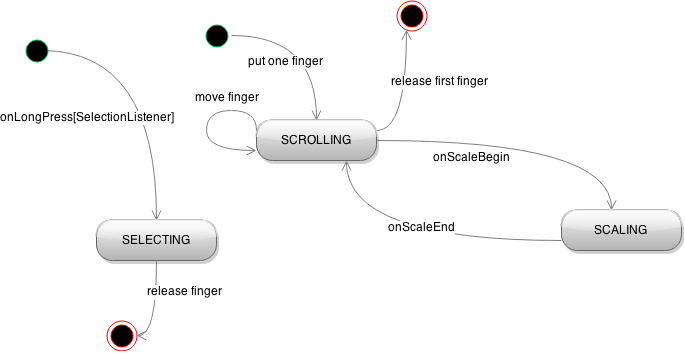
\includegraphics[scale = 0.5]{img/android/STATE_DIAGRAM}
      \caption{State diagram of the viewport.}
      \label{fig:viewport_state_diag}
     \end{figure}
    ~\\
    
 \begin{itemize}
  \item[$\rightarrow$] \textit{NONE} state  : The application doesn't have any state, the user is not doing anything;\\
  \item[$\rightarrow$] \textit{SELECTING} state : the user is selecting a square to send to the calibration server. The hovered square is colored in green. The long press begins when the user touches the screen without moving and wait like this for one second. Besides, in order to reach the '\textit{SELECTING}' state, the condition \textit{onLongPress[SelectionListener]} to the diagram to indicate that if the SelectionListener is null (the case in LocationViewport constructor), then it is naturally impossible to reach the SELECTING state.\\
  \item[$\rightarrow$] \textit{SCROLLING} state : the user is translating the map with one finger.\\
  \item[$\rightarrow$] \textit{SCALING} state : the user performs a classic scale with two fingers on the screen.\\
 \end{itemize}
    ~\\
\indent It is important to mention that there is no way of switching directly from the \textit{SCROLLING}/\textit{SCALING} states to the \textit{SELECTING} state and inversely. It is a choice made in order for the user to be able to scroll and scale without preoccupying himself on how long his finger did not move.

\subsubsection {Relativity}
    When the different states are defined, we have to handle relativity. Relativity in the application means that, if the user can zoom and translate the viewport, all graphical objects must have global coordinates (on the map, or the "world") and local coordinates (on the screen). \\
    
     \begin{figure}[H]
      \centering
       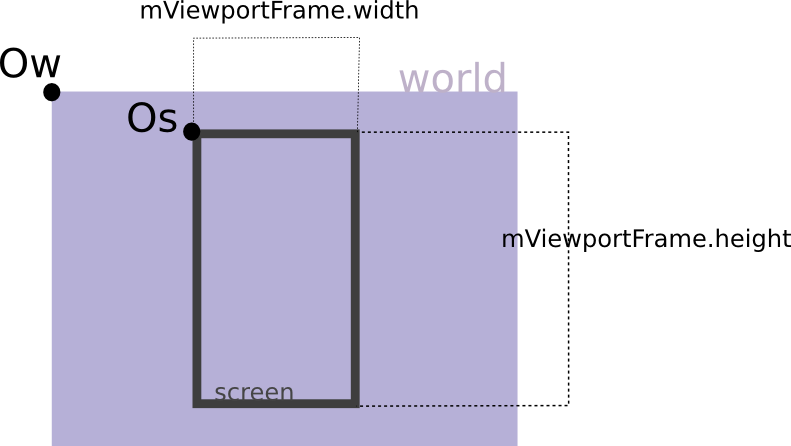
\includegraphics[scale = 0.5]{img/android/Viewport_relativity}
      \caption{Viewport relativity diagram.}
      \label{fig:viewport_relativity_diag}
     \end{figure}
    ~\\
    
     The \textbf {mViewportFrame} field is a RectF expressed in world coordinates. \textit{Ow} is the world origin (ie (0, 0)), and \textit{Os} is the mViewportFrame offset. This frame act like a screen avatar in the world system coordinates.
We defined also a \textbf {mScaleFactor} which is the ratio between the screen size (ie canvas size) and the mViewportFrame size. \\
\indent In order to make it more readable in the code, we created two indispensable functions which use these two elements (mViewportFrame and mScaleFactor) to convert points or distances:\\
    \begin{itemize}
     \item[$\rightarrow$] \textit{fromViewToWorld}();
     \item[$\rightarrow$] \textit{fromWorldToView}().
    \end{itemize}
    ~\\
\indent Either of them takes 2 coordinates as parameter and returns the transformed point as a PointF or as a distance (as a float value). Before creating these two methods, it was impossible to handle relativity problems with clarity.

   \subsubsection {Border limits of the viewport}
    Naturally, we had to introduce border limits in the application in order to offer more comfort for the user. Functions which handle this topic share the name  \textit{limitViewportToBounds}. They reset the mViewportFrame according to the bounds given in parameters.

   \subsubsection {The selection listener}
    The selection listener is an inner class which have to be given in the Viewport constructor if we want to handle a selection behavior. If it is null or not given, the \textit{SELECTING} state won't be reached. Indeed it is the case in Location viewport, where the user is not able to select a square.
 
  \subsection{WorldMap part}

 \begin{sidewaysfigure}
     \rotatebox{0}{
      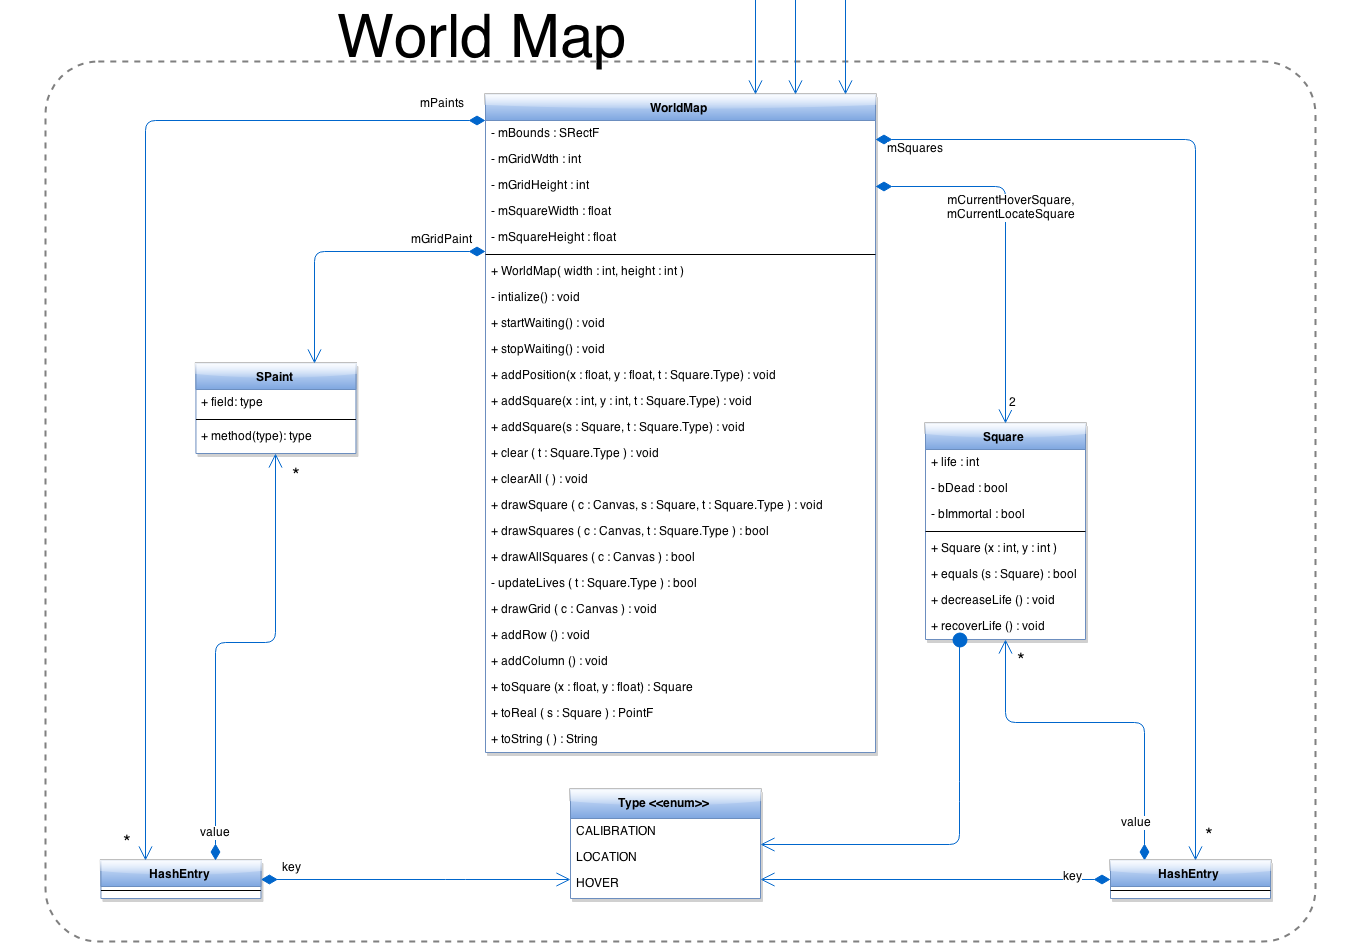
\includegraphics[scale=0.5]{img/android/LO53_Android_Class_WorldMap} }
     \caption{Class diagram representing the WorldMap.}
      \label{fig:worldmap_class_diag}
     \end{sidewaysfigure}
    \newpage
   ~\\
   
      This class his handled to store and draw squares. There are 3 types of squares : \textit{CALIBRATION}, \textit{LOCATION}, and \textit{HOVER}.  \\
\indent Each square contains a \textit{life} property which is used to handle a fade out behavior : Calibration squares are set as immortal, they are always drawn and never fade out whereas Location and Hover squares are mortal, they fade out if they are not the last added one.\\
 \section{Choices made and relevant details}
  \subsection {Modifying the settings only at the beginning}
  We decided to disable the modification of the settings when either calibration or location have been launched because we wanted to have a certain consistency in the project. If we could change server IP between calibration and location sessions, it would have quickly confused the application. Moreover we use a unique server IP for both so it would have been totally irrelevant and useless to permit the application changing it when running.
  \subsubsection {A persistent map common to all fragments}
  As described in the purpose part, the world map has to be unique for all the application, it also has to : 
  \begin{itemize}
  \item[$\rightarrow$] be persistent : it means that if we let the program run in background or if we let the screen turn off, the map should not be removed;
  \item[$\rightarrow$] be able to be shared to all fragments from the main activity.
  \end{itemize}
  ~\\
\indent There are several ways to do such things and the one selected is very efficient as it can do both, we are talking about the \textbf{Bundle}.

\paragraph{Bundle}
The aim of the Bundle class is to store data in order to serialize/deserialize it later. To store data inside, we instantiate it and insert data with a put function : for example we used here putSerializable :
\textit{mMapSaveBundle.putSerializable(TAG\_WORLDMAP, new WorldMap(width, height));} \\
\indent It takes :
   \begin{itemize}
    \item[$\rightarrow$] a string tag, which is here a static field of MainActivity;
    \item[$\rightarrow$] the serializable object that we want to put in.
   \end{itemize}
   ~\\
\paragraph{Share a Bundle}
    When we create a map bundle and in order to share it, we can use the \textit{setArguments()} and \textit{getArguments()} fragment's functions. \textbf{In activity} : we call the \textit{setArguments( Bundle bundleToShare)} function just before replacing the fragment container, because the bundle argument has to be set before the call of \textit{onCreateView()} fragment's function. \textbf{In fragment} : precisely in the \textit{onCreateView()} function, we call \textit{getArguments()} function to retrieve the bundle.

\paragraph{Store a Bundle}
    When the application is run in background, when we touch the home button or even when the screen turns on, the main activity is instanciated again. So we have to save what we called the persistent data (ie. the map) in order not to flush the data already gathered. It needed to override two activity's functions to save or restore : 
    \begin{itemize}
    \item[$\rightarrow$] \textit{onSaveInstanceState(Bundle savedInstanceState)};
    \item[$\rightarrow$] \textit{onRestoreInstanceState(Bundle savedInstanceState)};
    \end{itemize}
    ~\\
    What is interesting here is that we can put a bundle inside a bundle. In this way, we can save the map bundle inside the savedInstanceState bundle.
  
  \subsubsection {Preference settings more persistent}
   We could have used again a bundle to handle the user preferences, but at each launch of the application, the savedInstanceState bundle is flushed. This is why android provides something largely more attractive for this kind of persistent data : the SharedPreferences. These are stored into the mobile phone and so will persist even if we close the app.
  
  \subsubsection {Data reception in the Location fragment}
   As we saw, the location has to make a loop with send and receive statements. The problem here is a classic synchronization problem. As we have a viewport which can be dragged and scaled, the reception could not be performed in the same thread. If it was the case, the socket would wait for positions to receive, blocking the thread and so disabling for a moment the drag and scale possibilities. That is why we had to make the reception asynchronous.\\ 
\indent We first thought of creating a thread, assign it a runnable Receiver and simply run it. But this is not how it is supposedly done through the Android API because of specific threading behaviors already running. Android discourages the creation of our own threads and provides a very efficient tool : the asynchronous task. It is efficient because we don't have to manage Thread or UIThread, etc ... and it provides a code as clear as possible. 

  \subsubsection {Two detectors to handle two input types}
  There are ways to handle both scale and scroll inputs using only the scale gesture detector, but when we look at the functions provided by its interface listener, we see that it has not been done in this aim. Unlike the gesture detector interface which contains functions like \textit{onScrolling}, \textit{onLongPress}, or \textit{onSingleTap} which are very useful to handle events. This is why we decided to take advantages from both and use a scale gesture detector to retrieve scale input and a gesture detector to retrieve scroll input.

  \section{User guide}
The first screen the user sees is the setting screen. Here are the parameters the user can modify :
\begin{itemize}
 \item[$\rightarrow$] "Use the server" : Define if we really use a server or if we want a randomly simulated server. Basically it is quite useful for debug, when we have not necessarily a sever at proximity.
 \item[$\rightarrow$] "Server IP" : the IP of the server to connect to.
 \item[$\rightarrow$] "Location Port" : the port used by the server for location requests.
 \item[$\rightarrow$] "Calibration Port" : the port used by the server for calibration requests.
 \item[$\rightarrow$] "Default map width" : the width (in squares) of the map shown to the user.
 \item[$\rightarrow$] "Default map height" : the height (in squares) of the map shown to the user.
\end{itemize}
  
\begin{figure}[H]
    \centering
      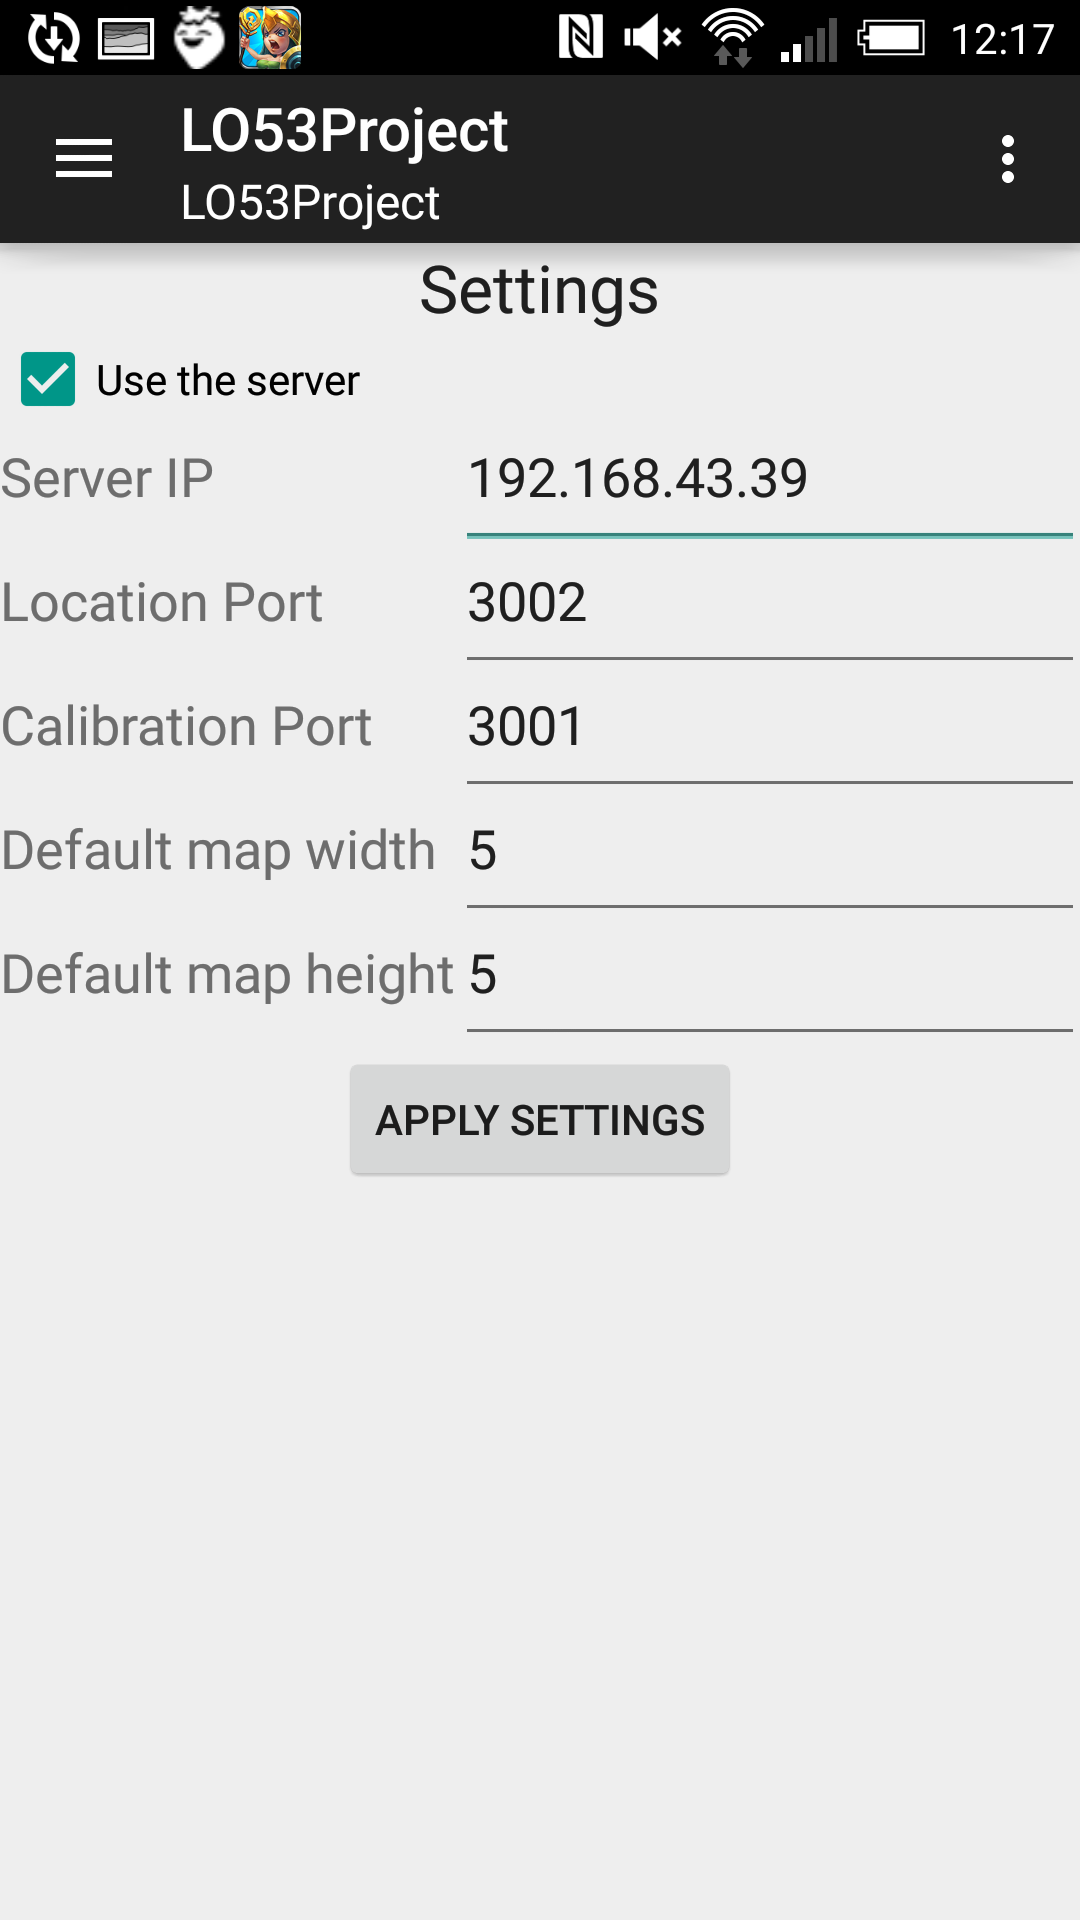
\includegraphics[scale=0.15]{img/android/Settings_SC}
        \caption{Settings screenshot.}
        \label{fig:settings_sshot}
\end{figure}
~\\

\indent When the user is satisfied with the settings, he has to click on the Apply Settings button, or the program will not take in count the changes. Beware, the settings can only be changed at the beginning of the program. Moreover, the next time the program is run, the newly created settings will be proposed.\\
\indent The next step is to select either the calibration mode (if we want to make a fingerprint) or the location mode (if we just want to see our position). If no fingerprint have been registered yet, the location part will not be able to make any requests. The selection is done in the selector button upper left :

    \begin{figure}[H]
     \centering
      
\includegraphics[scale=0.3]{img/android/Selector_button}
     \caption{Selector button.}
     \label{fig:select_button}
    \end{figure}
    ~\\

\subsubsection {Location :}
    There is nothing specific to do here, just see your position in the room, represented by a white square on the map. The last position received is totally opaque, and fades with time.
    
\begin{figure}[H]
    \centering
      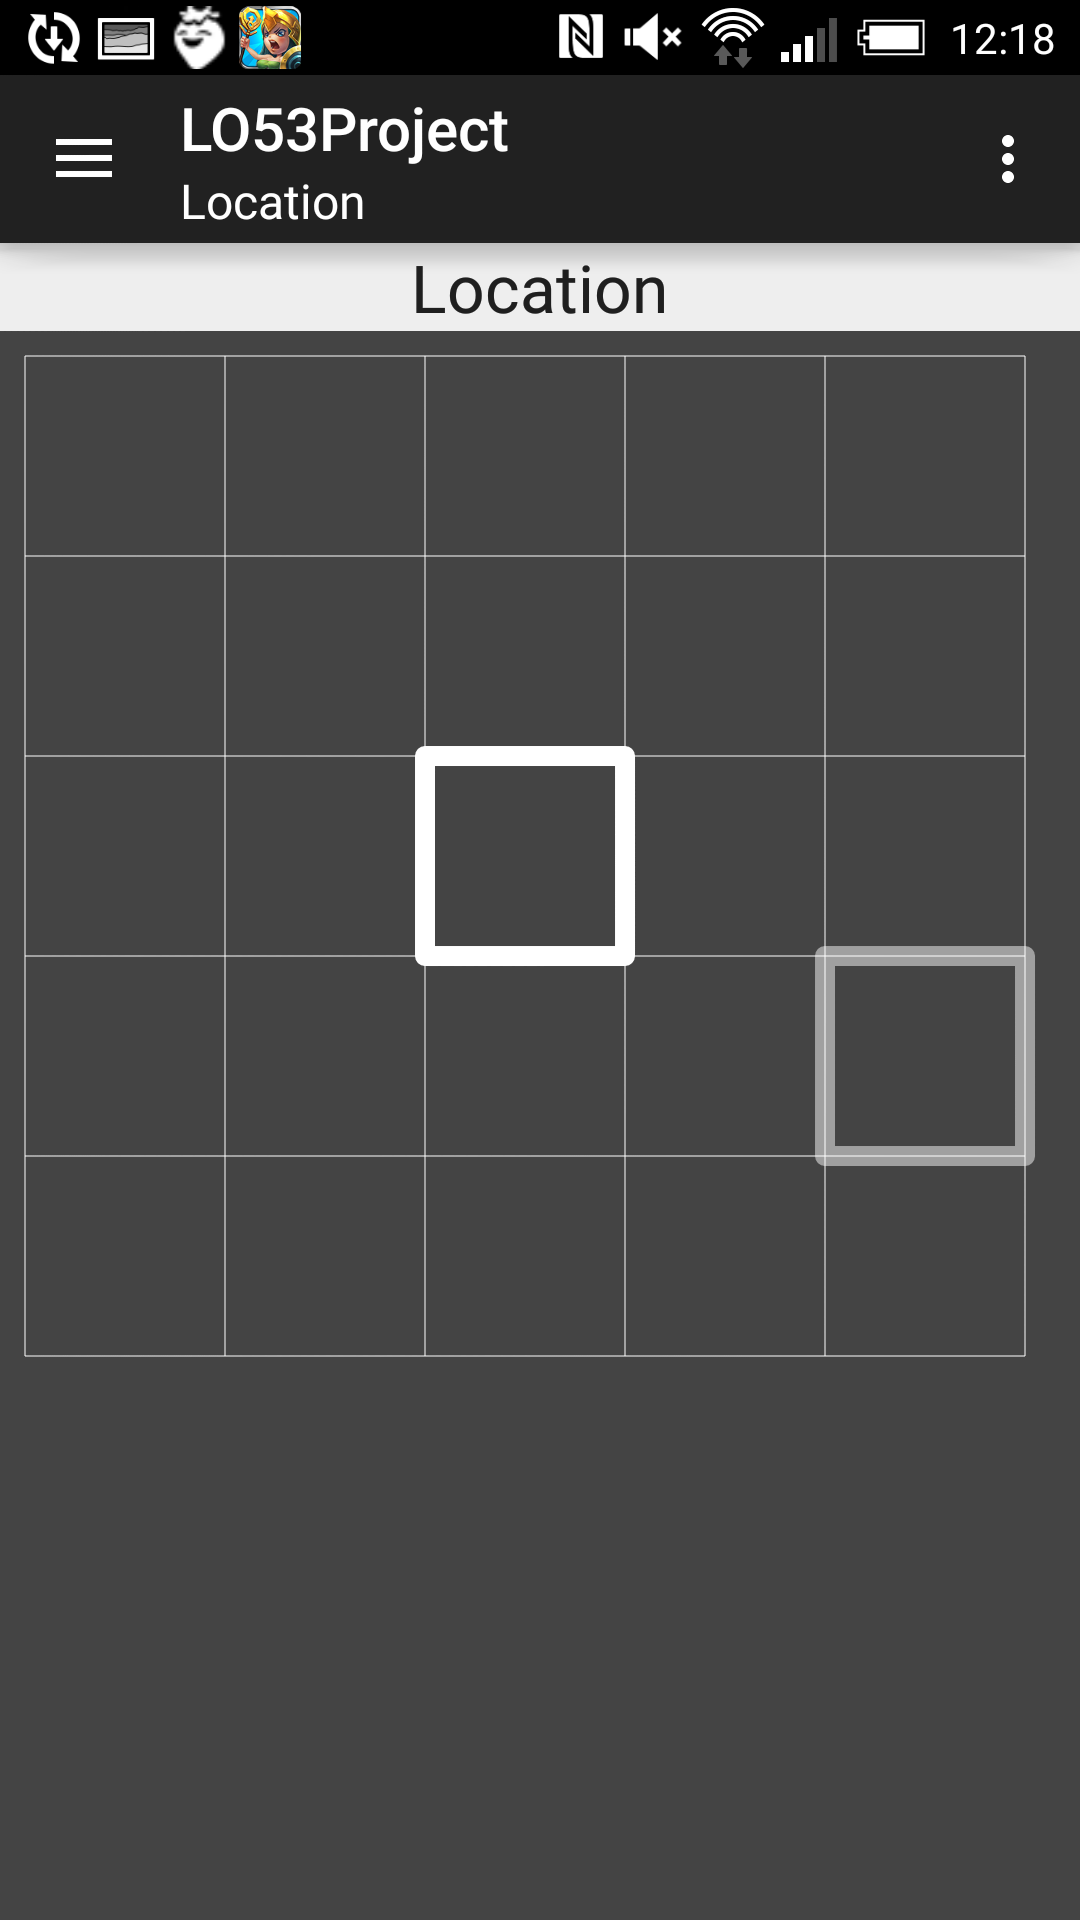
\includegraphics[scale=0.15]{img/android/Location_SC}
        \caption{In location : White squares represent our position.}
        \label{fig:location_sshot}
\end{figure}
~\\

\newpage
\subsubsection {Calibration :}
    First of all, the user can add a column or a row to the map by performing a single tap respectively on the vertical or the  horizontal white "button".

	\begin{figure}[H]
     \centering
     \begin{minipage}{.5\textwidth}
	  \captionsetup{width=.7\textwidth}
      \centering
      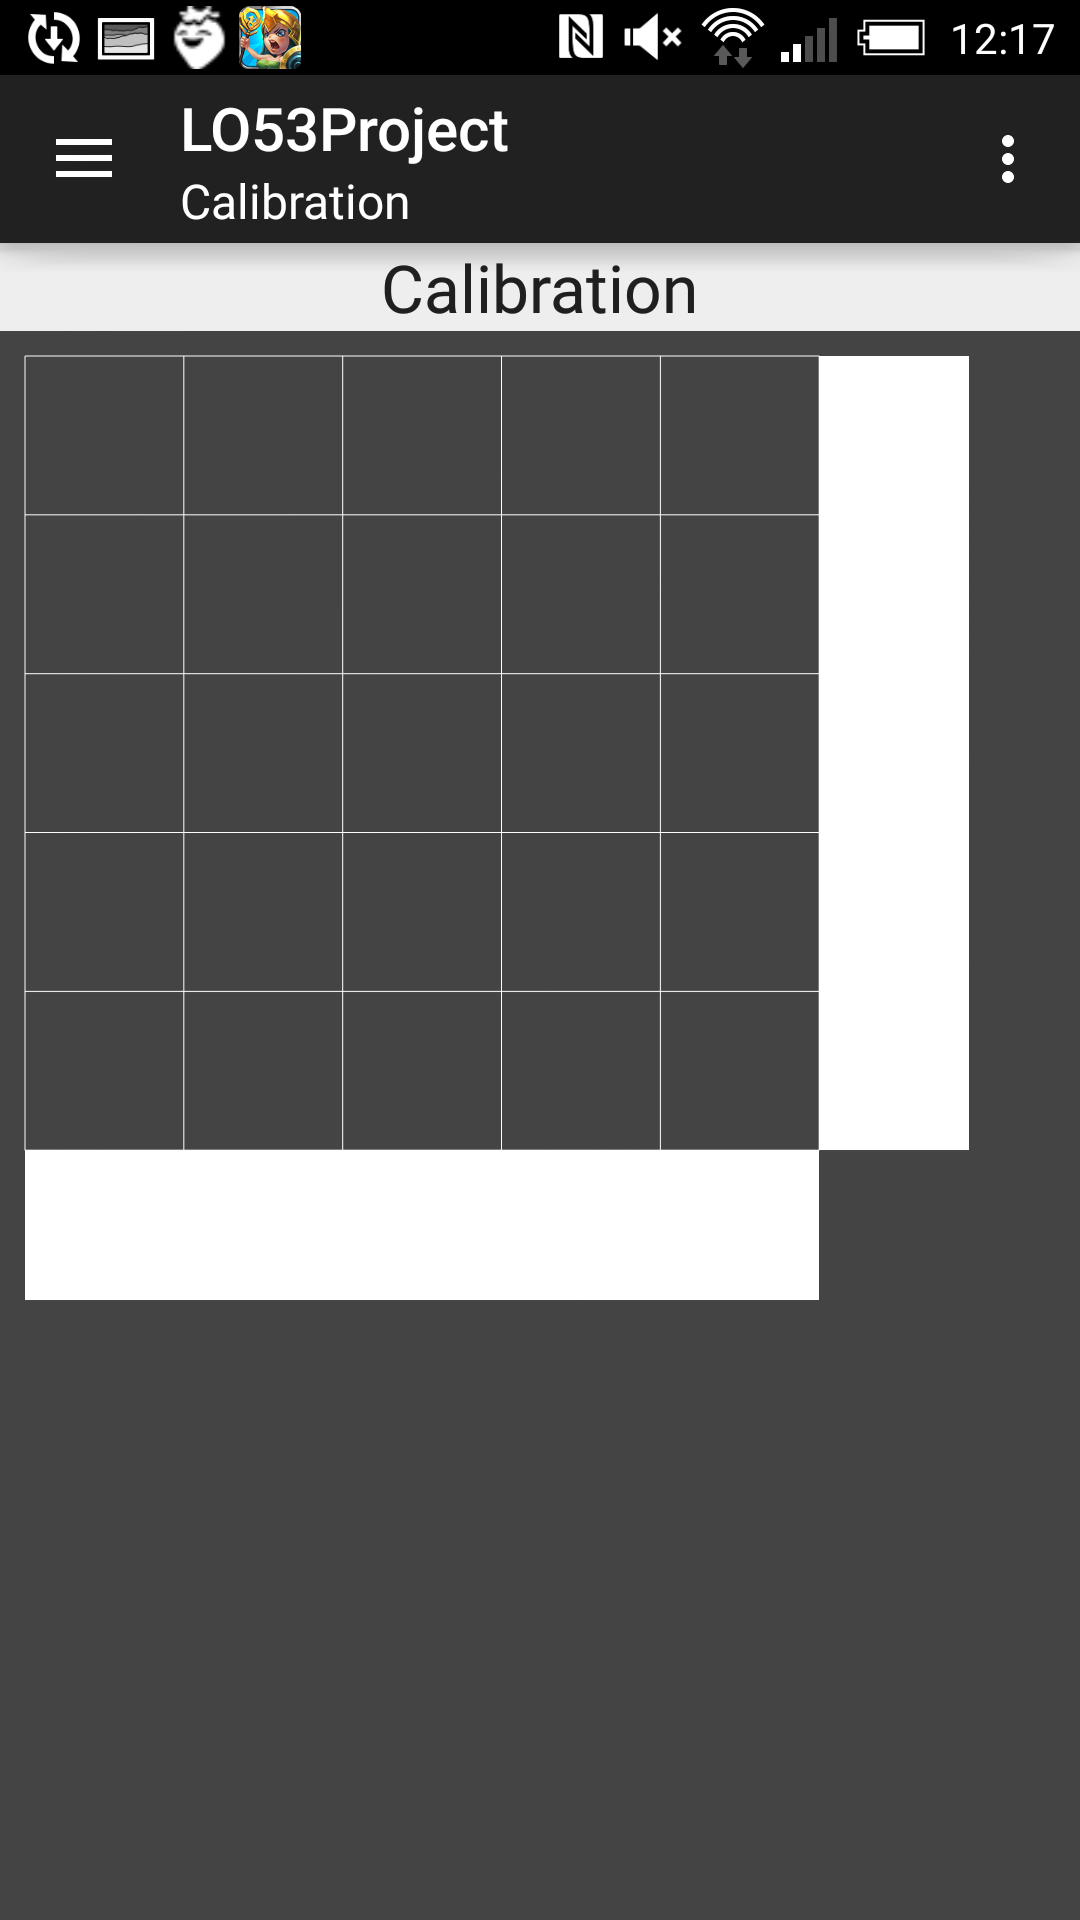
\includegraphics[scale=0.1]{img/android/Calibration_AddCol1}
        \caption{In calibration : Before add a row}
        \label{fig:calib_bef_sshot}
     \end{minipage}%
     \begin{minipage}{.5\textwidth}
	  \captionsetup{width=.7\textwidth}
	  \centering
      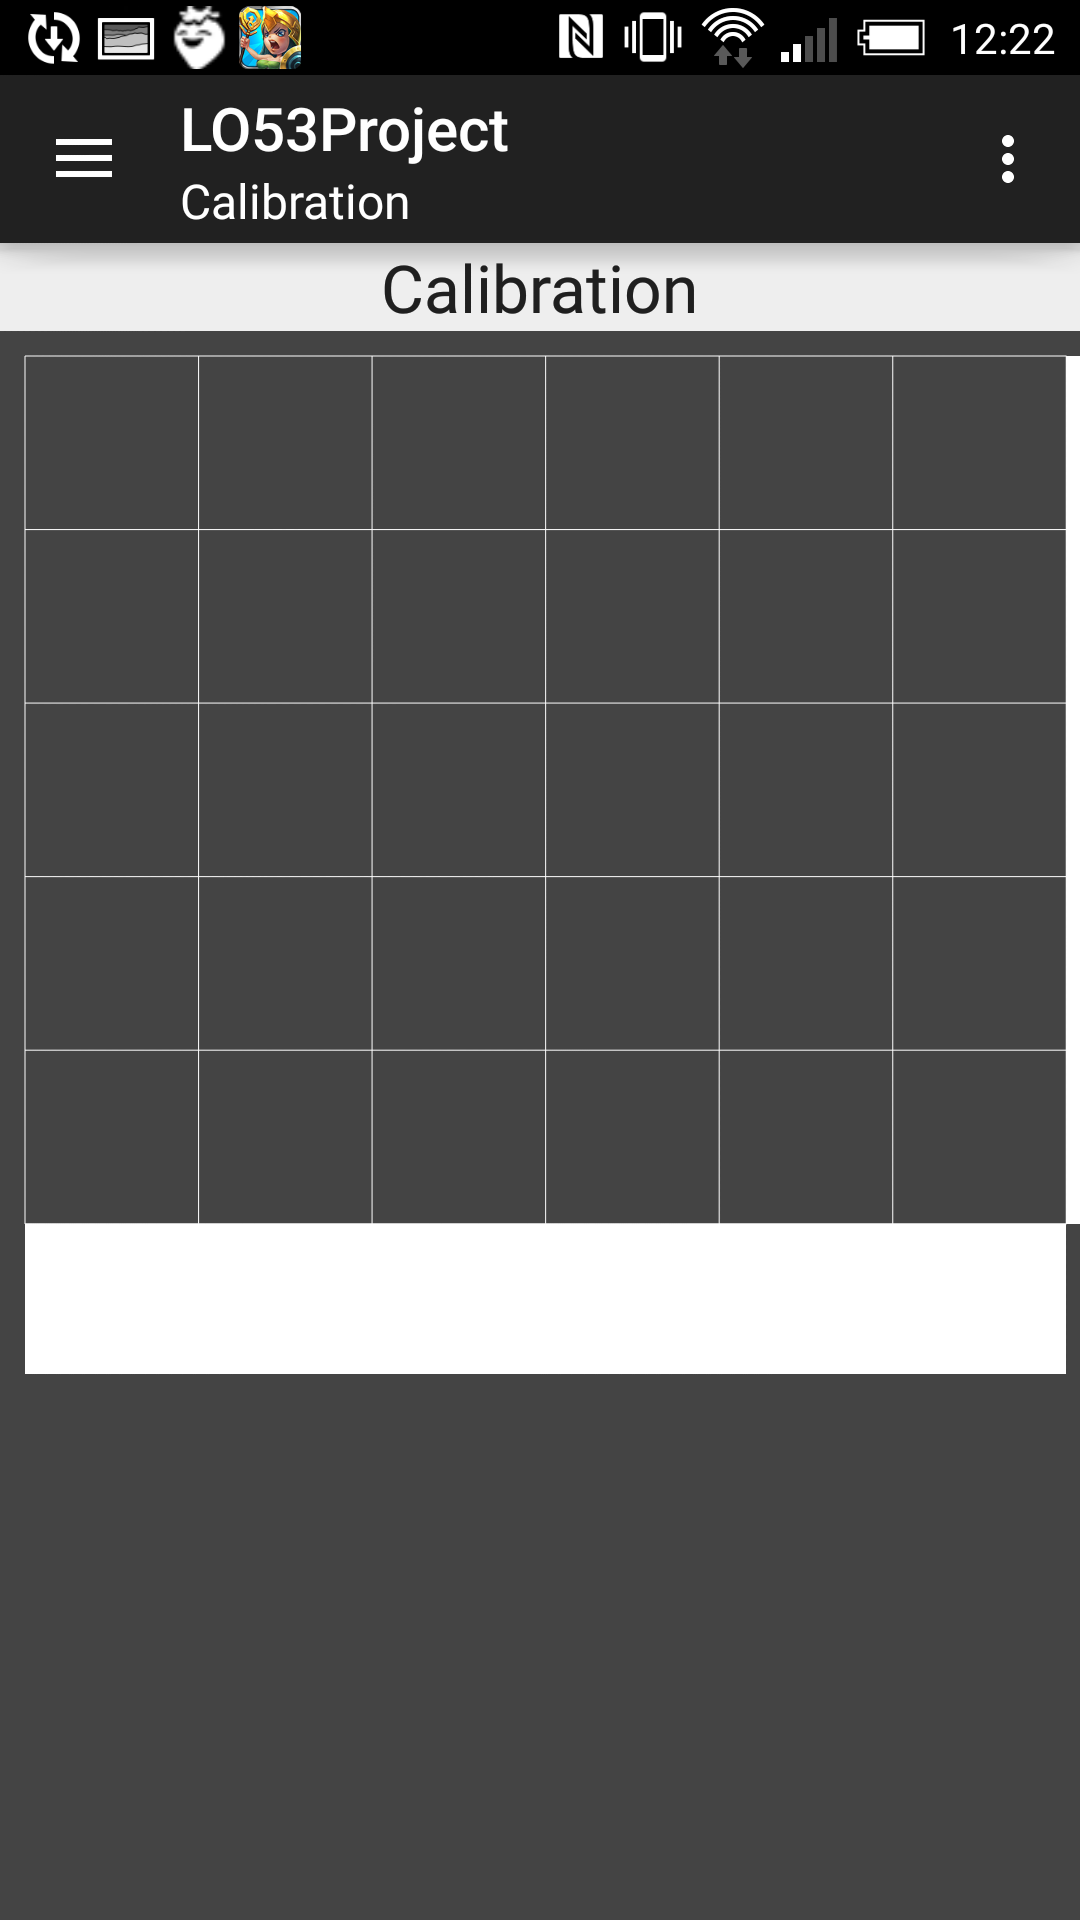
\includegraphics[scale=0.1]{img/android/Calibration_AddCol2}
        \caption{In calibration : After add a row}
        \label{fig:calib_aft_sshot}
     \end{minipage}
    \end{figure}

~\\
\indent Secondly, and the most important, you can add a calibration position. To do this, select a square by touching it without moving during one second. When the square is filled with green and if you did not release your finger, you can even move across the map while sliding your finger. 

	\begin{figure}[H]
     \centering
     \begin{minipage}{.4\textwidth}
	  \captionsetup{width=.7\textwidth}
      \centering
        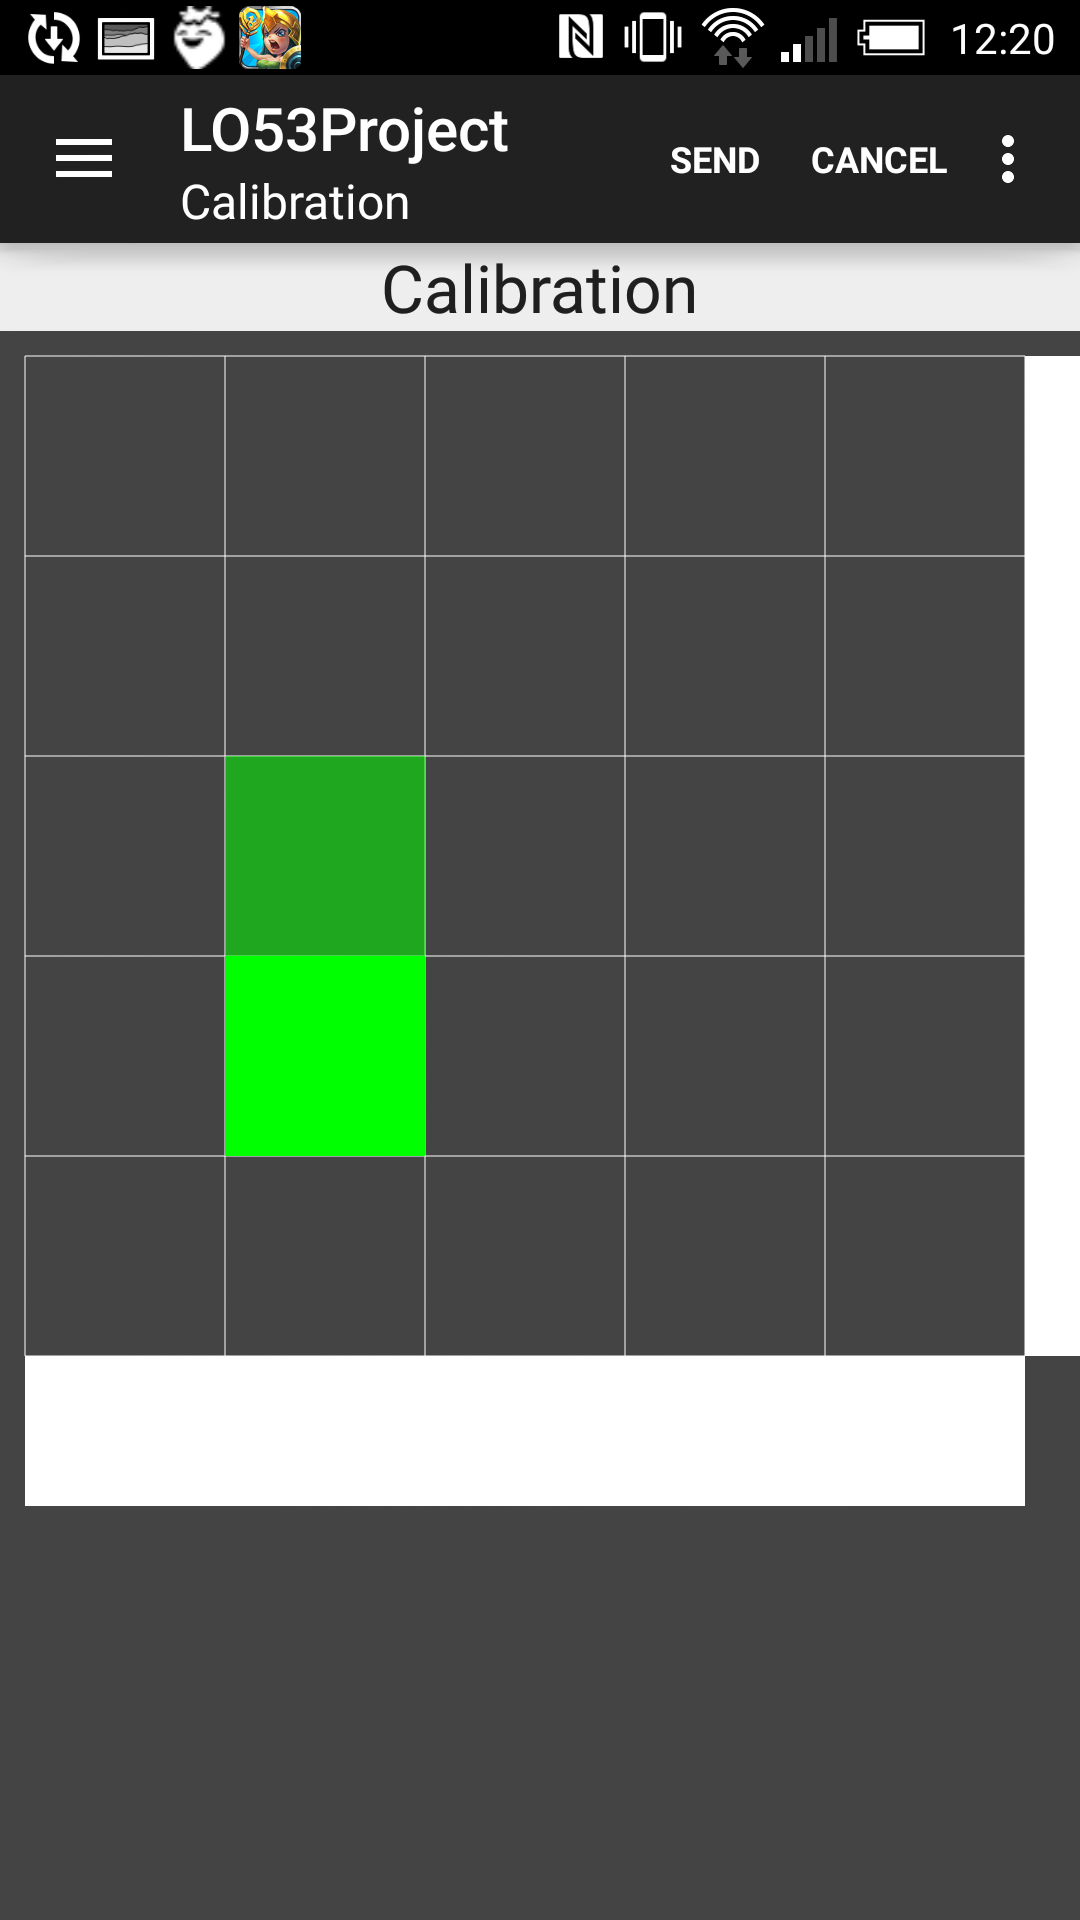
\includegraphics[scale=0.1]{img/android/Calibration_select1}
        \caption{In calibration : Selection in progress.}
        \label{fig:calib_sel1_sshot}
     \end{minipage}
     \begin{minipage}{.4\textwidth}
      \captionsetup{width=.7\textwidth}
      \centering
      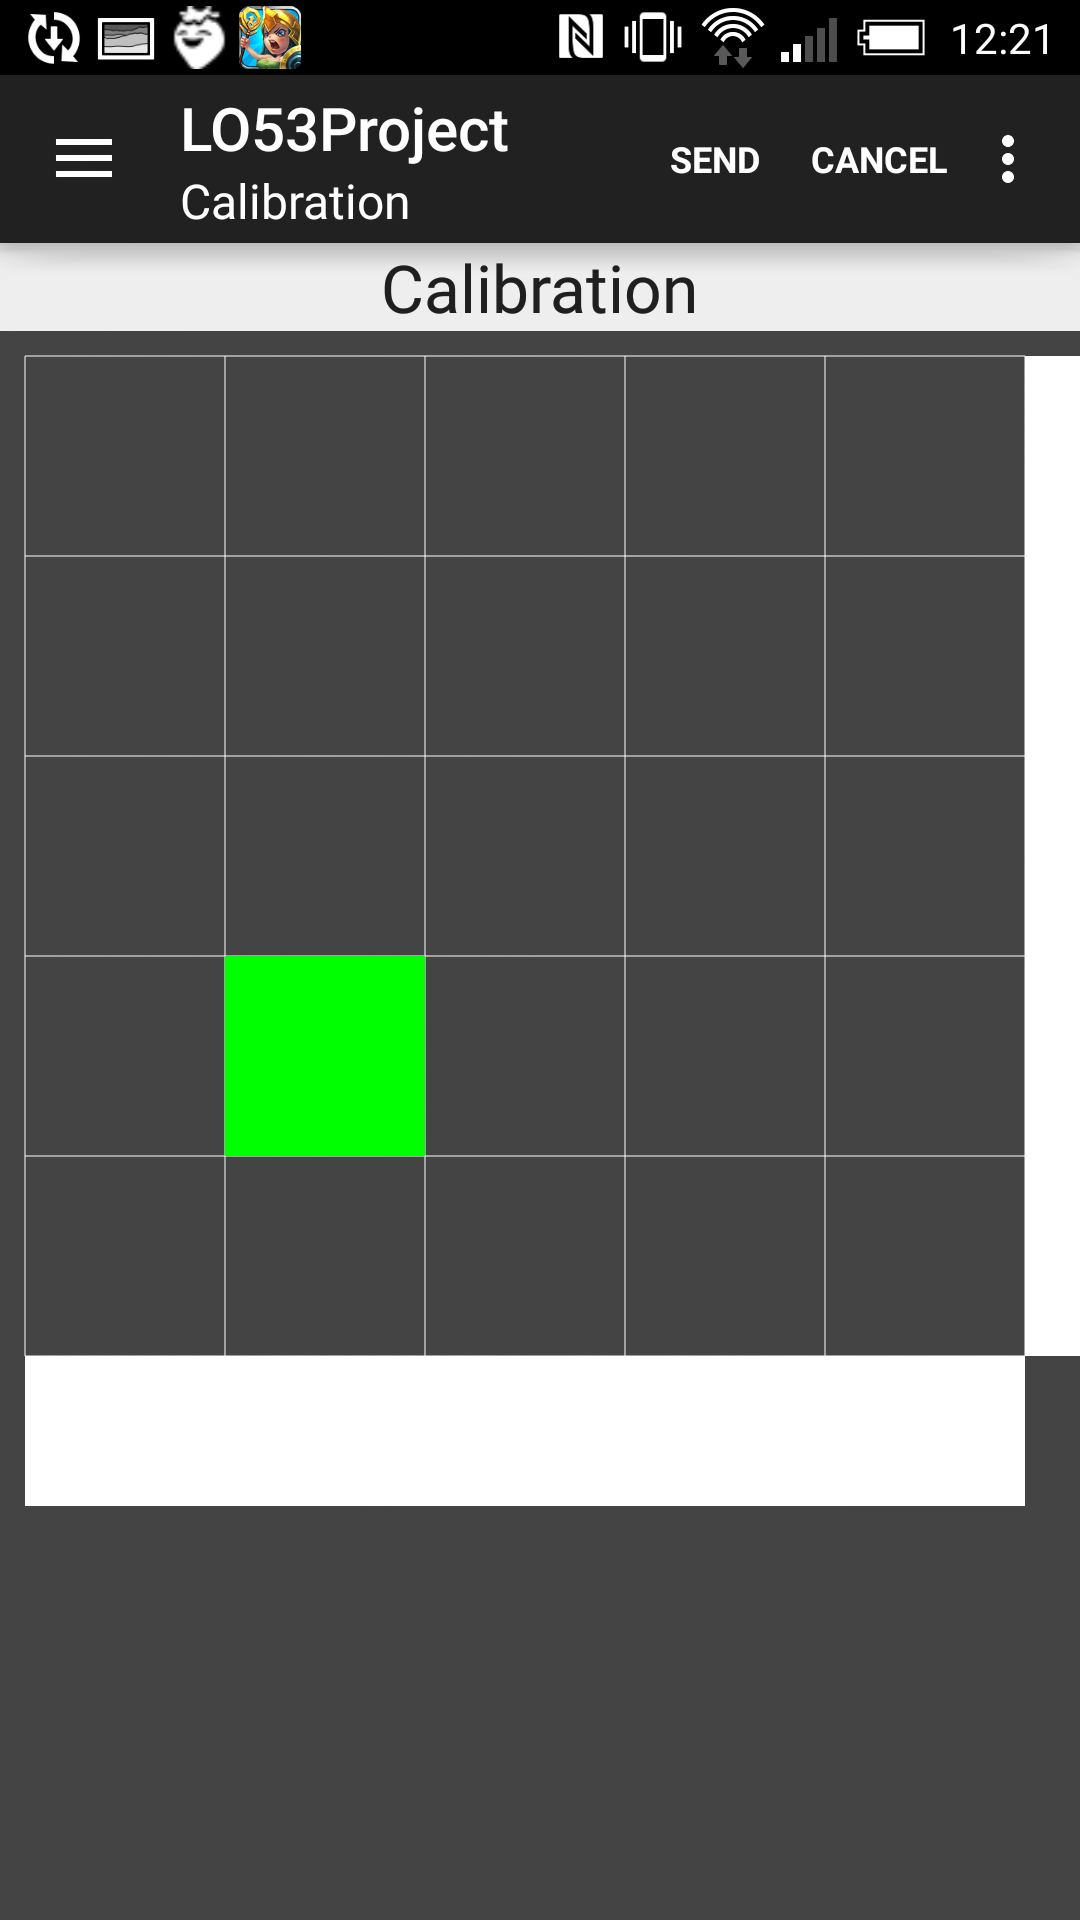
\includegraphics[scale=0.1]{img/android/Calibration_select2}
      \caption{In calibration : Selected square persists after finger release}
       \label{fig:calib_sel2_sshot}
     \end{minipage}
    \end{figure}

~\\
\indent When you are satisfied by the square you selected (ie. it corresponds to your current real position) you can send it to the server with the 'Send' button on the top of the screen. If you are not satisfied, you can either use the 'Cancel' button, or select another square just like before.

\begin{figure}[H]
    \centering
      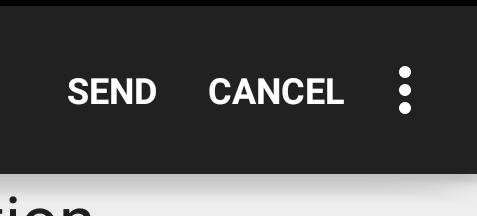
\includegraphics[scale=0.3]{img/android/SendCancel_buttons}
        \caption{Send and Cancel buttons.}
        \label{fig:send_cancel_button_sshot}
\end{figure}
~\\
\indent When you send the point, and if the server has well received the point, a message is shown and the square is displayed in black. \\
\indent Eventually, in both calibration and location mode, you can translate or zoom the map respectively with one or two fingers the usual way.

  \section{Ameliorations}
  The application could certainly be more accurate on the positions given to the user. For example by asking to him : 
  \begin{itemize}
   \item[$\rightarrow$] a referential point which defines the map center;
   \item[$\rightarrow$] a custom geographic scale (ie. width and height of each square corresponds to how many real life meters) decided beforehand by the user. This would improve the precision between the simulated grid map and the real world open space.
  \end{itemize}
  ~\\
\indent Honestly, the graphical design is very poor, not to say non-existent. This is also a point which can be largely improved. We concentrated our efforts on something able to be run and to work, not something beautiful.\\
\indent In the end, there still are some problems with the zoom limit : unzooming quickly doesn't limit correctly the scale factor.  